% 2008 年陕西卷文科第 19 题：三棱锥被平行于底面 ABC 的平面截得的几何体，
%   截面 A1B1C1，∠BAC=90°，A1A⊥平面 ABC，A1A=√3，AB=AC=2A1C1=2，D 为 BC 中点。
% 来源 PDF：gaokaomath-src/普通高考/2008/2008陕西文.pdf
% SHA-256：a0e35ce2cc6835012265595cf3b3fefa10f81e868623d594f4dddc786905c6ad
% 原页：2008陕西文.pdf 第 1 页（A3 三栏）第 3 栏，书页码 477。
% 重绘依据：按原页斜投影画截头棱台状几何体：下底 ABC、上底 A1B1C1（相似比 1/2），
%   A1 在 A 正上方，侧棱 AA1、BB1、CC1 为实线；AD 为底面内中线，用虚线。
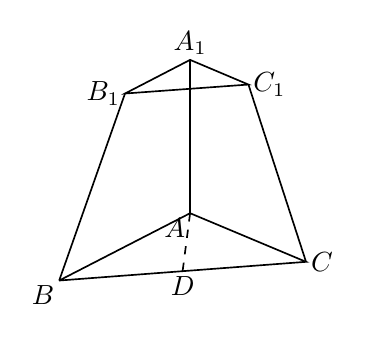
\begin{tikzpicture}[scale=0.95, semithick, every node/.style={inner sep=1.5pt}]
  \coordinate (A) at (1.05,1.00);
  \coordinate (B) at (-0.70,0.10);
  \coordinate (C) at (2.60,0.35);
  \coordinate (D) at (0.95,0.225);
  \coordinate (A1) at (1.05,3.05);
  \coordinate (B1) at (0.18,2.60);
  \coordinate (C1) at (1.83,2.72);

  \draw (B) -- (A) -- (C) -- (B);
  \draw[dashed] (A) -- (D);
  \draw (A) -- (A1);
  \draw (B) -- (B1);
  \draw (C) -- (C1);
  \draw (A1) -- (B1) -- (C1) -- cycle;

  \node[below left] at (A) {$A$};
  \node[below left] at (B) {$B$};
  \node[right] at (C) {$C$};
  \node[below] at (D) {$D$};
  \node[above] at (A1) {$A_1$};
  \node[left] at (B1) {$B_1$};
  \node[right] at (C1) {$C_1$};
\end{tikzpicture}
